\documentclass[oneside]{book}
\usepackage{epsfig,graphicx} % Required for inserting images
\usepackage{amsmath}
\usepackage{amsthm}
\usepackage{amssymb}
\usepackage{subcaption}
\usepackage[spanish,mexico]{babel}
\usepackage[bookmarksopen]{hyperref}
\usepackage[utf8]{inputenc}
\usepackage{array}
\usepackage{listings} %Soporte para código
\usepackage[left=2cm,right=2cm,top=1.8cm,bottom=2.3cm]{geometry}

%\usepackage{schemata}
% ---definición de los paquetes--
\usepackage{fancyhdr}            % Permits header customization. See header section below.
\fancypagestyle{plain}{
    \lhead{}
    \fancyhead[R]{\thepage}
    \fancyhead[L]{}
    \renewcommand{\headrulewidth}{0pt}
    \fancyfoot{}
}
\pagestyle{fancy}
\fancyhead[R]{\thepage}
\fancyhead[L]{}
\title{Tarea 01: Naturales, inducción y recursión}
\author{Ramírez Mendoza Joaquín Rodrigo\\
Villalobos Juárez Gontran Eliut\\
Treviño Puebla Héctor Jerome}
\date{\today}
% ---Inicio de la portada
\begin{document}

    \begin{titlepage}

    \begin{minipage}{3cm}
    	\begin{center}
    		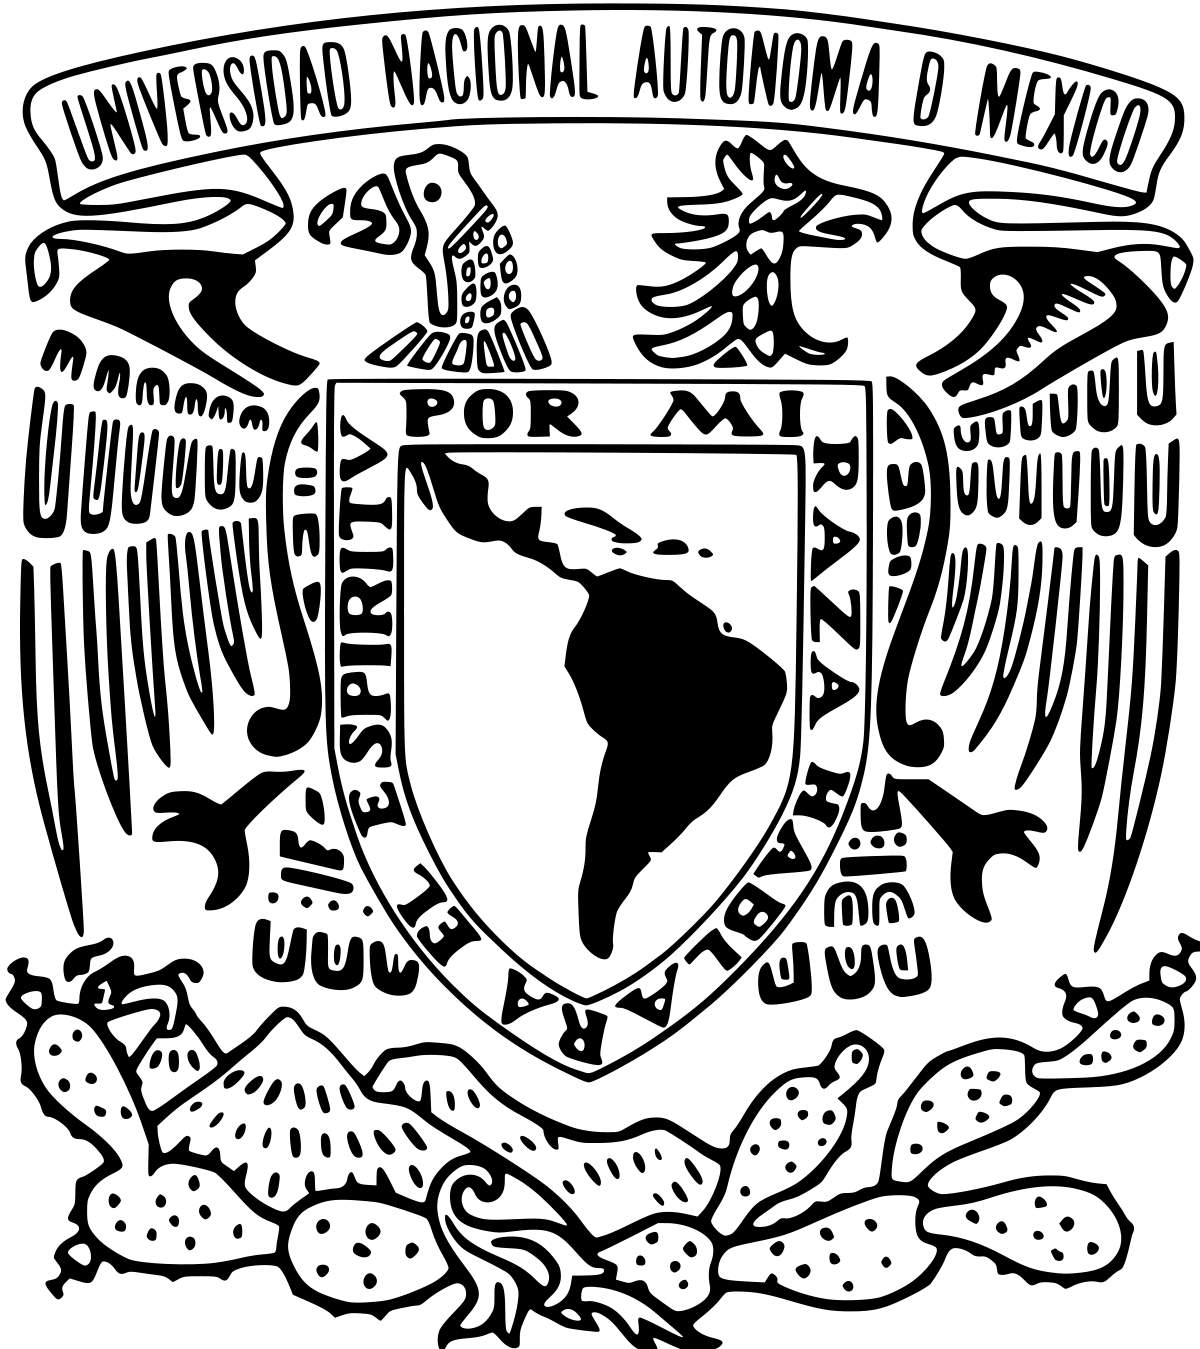
\includegraphics[height = 0.14\textheight]{recursos/Logo_UNAM.png}\par
    	\end{center}
    \end{minipage}\hfill
    \begin{minipage}{10cm}
    	
    \end{minipage}\hfill
    \begin{minipage}{3cm}
    	\begin{center}
    		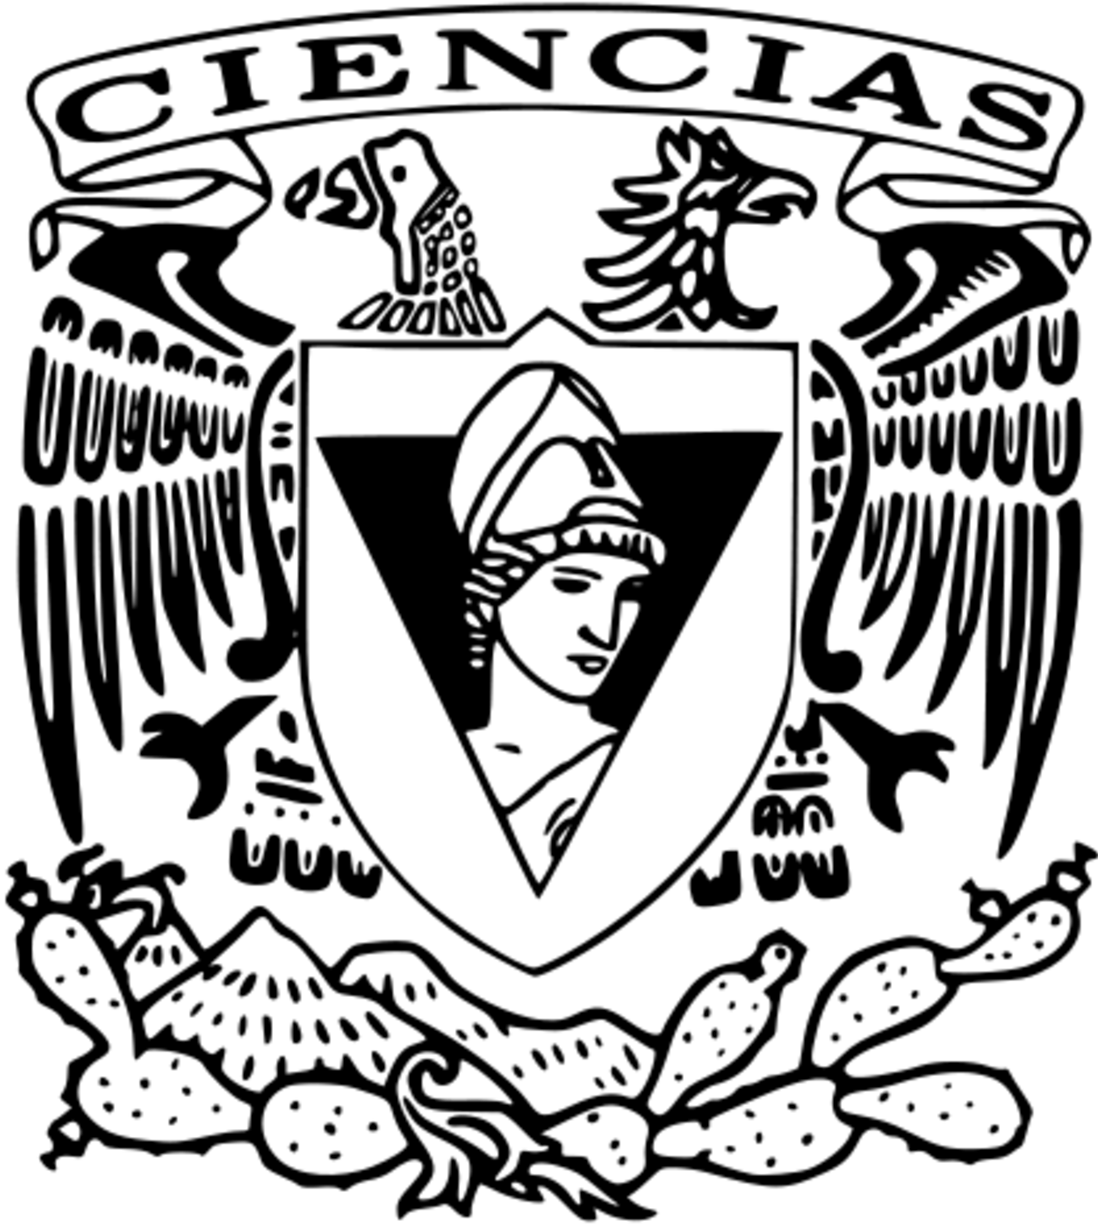
\includegraphics[height = 0.14\textheight]{recursos/Logo_FC.png}\par
    	\end{center}
    \end{minipage}
        \centering
        \vspace{1cm}
        
        {\bfseries\LARGE Universidad Nacional Autónoma de México \par}
        
        \vspace{1cm}
        {\scshape\Large Facultad de Ciencias \par}
        \vspace{1cm}
        {\scshape\Large Estructuras Discretas \par}
        \vspace{1cm}
        {\scshape\Large Licenciatura en Ciencias de la Computación \par}
        \vspace{1cm}
        {\scshape\Huge Tarea 01: Naturales, inducción y recursión.  \par}
        \vspace{3cm}
        {\itshape\Large Primer Parcial \par}
        \vfill
        {\Large Autores: \par}
        {\Large Ramírez Mendoza Joaquín Rodrigo \par}
        {\Large Villalobos Juárez Gontran Eliut\par}
        {\Large Treviño Puebla Héctor Jerome \par}
        \vfill
        {\Large Agosto 2024 \par}
    \end{titlepage}
% ---Fin de la portada de la portada
    \maketitle

% Introducir aquí sus capítulos
% ------∨∨∨∨∨∨∨∨∨∨∨∨∨∨∨--------
\textbf{1.-}\ Demostrar por inducción que para todo natural \textit{n}\ se cumple la siguiente igualdad:
\[
\sum_{k=0}^{n}2^k = 2^{n+1}-1
\]
Demostración por Inducción sobre \textit{n}\\
\newline
\textbf{1) Caso Base:}\ \textit{n=0}\
\[
\sum_{k=0}^{0}2^k = 2^{0+1}-1 
\]
\[
\ 2^{0}= 2^{1}-1
\]
\[
\ 1 = 1
\] 
\textbf{2) Hipótesis de Inducción:}\  Se cumple para \textit{n}\
\[
\sum_{k=0}^{n}2^k = 2^{n+1}-1
\]
\textbf{3) Paso Inductivo:}\  Por demostrar que se cumple para \textit{n+1}\
\[
\sum_{k=0}^{n+1}2^k = 2^{(n+1)+1}-1
\]
\[
\sum_{k=0}^{n+1}2^k = 2^{n+2}-1
\]
\[
\sum_{k=0}^{n}2^k + 2^{k+1} = 2^{n+2}-1
\]
\begin{center}
\textbf{Por H.I.} $\sum_{k=0}^{n}2^k = 2^{n+1}-1$ 
\end{center}
\[
2^{n+1} - 1 +2^{n+1} = 2^{n+2}-1
\]
\[
2^{1}(2^{n+1}) - 1 = 2^{n+2}-1
\]
\[
2^{(n+1)+1} -1 = 2^{n+2}-1
\]
\[
2^{n+2} - 1= 2^{n+2}-1
\]
\newline
\textbf{Por lo tanto} Demostramos que se cumple para toda \textit{n} que: 
\[
\sum_{k=0}^{n}2^k = 2^{n+1}-1
\]
\newpage

\textbf{2.-}\ Demostrar que para todo natural \textit{n}\ se cumple la igualdad:
\[
\sum_{k=0}^{n}k(k+1) = \frac{n(n+1)(n+2)}{3}
\]
Demostración por Inducción sobre \textit{n}\
\newline
\textbf{1) Caso Base:}\ \textit{n=0}\
\[
\sum_{k=0}^{0}k(k+1) = \frac{0(0+1)(0+2)}{3}
\]
\[
0(0+1) = \frac{0(1)(2)}{3}
\]
\[
0(1) = \frac{0}{3}
\]
\[
0 = 0
\]
\textbf{2) Hipótesis de Inducción:}\  Se cumple para \textit{n}\
\[
\sum_{k=0}^{n}k(k+1) = \frac{n(n+1)(n+2)}{3}
\]
\textbf{3) Paso Inductivo:}\  Por demostrar que se cumple para \textit{n+1}\
\[
\sum_{k=0}^{n+1}k(k+1) = \frac{(n+1)((n+1)+1)((n+1)+2)}{3}
\]
\[
\sum_{k=0}^{n+1}k(k+1) = \frac{(n+1)(n+2)(n+3)}{3}
\]
\[
\sum_{k=0}^{n}k(k+1) + (n+1)((n+1)+1) = \frac{(n+1)(n+2)(n+3)}{3}
\]
\[
\sum_{k=0}^{n}k(k+1) + (n+1)(n+2) = \frac{(n+1)(n+2)(n+3)}{3}
\]
\begin{center}
\textbf{Por H.I.} $\sum_{k=0}^{n}k(k+1) = \frac{n(n+1)(n+2)}{3}$ 
\end{center}
\[
\frac{n(n+1)(n+2)}{3} + (n+1)((n+2) = \frac{(n+1)(n+2)(n+3)}{3}
\]
\[
\frac{n(n+1)(n+2) + 3(n+1)(n+2)}{3} = \frac{(n+1)(n+2)(n+3)}{3}
\]
\[
\frac{(n+1)(n+2)(n+3)}{3} = \frac{(n+1)(n+2)(n+3)}{3}
\]
\newline
\textbf{Por lo tanto} Demostramos que se cumple para toda \textit{n} que: 
\[
\sum_{k=0}^{n}k(k+1) = \frac{n(n+1)(n+2)}{3}
\]\newpage
\textbf{3.-}\ Para todo $n \in N$ se tiene que $2^{2n} -1 $ es múltiplo de $3$.\\
\newline
Demostración por Inducción sobre \textit{n}\
\newline
\textbf{1) Caso Base:}\ \textit{n=0}\
\[
2^{2(0)}-1
\]
\[
2^{0}-1
\]
\[
1-1
\]

\[
\frac{0}{3} = 0
\]
\[
0
\]
\newline
$0$ es múltiplo de 3, se cumple el Caso Base.\\
\newline
\textbf{2) Hipótesis de Inducción:}\  La propiedad se cumple para \textit{n}\
\begin{center}
$2^{2n}-1$ es Múltiplo de 3
\end{center}
\[
\frac{2^{2n} - 1}{3} \in N
\]
\textbf{3) Paso Inductivo:}\  Por demostrar que se cumple para \textit{n+1}\
\[
2^{2(n+1)} - 1
\]
\[
2^{2n+2} -1
\]
\[
(2^{2n})(2^{2}) - 1
\]
\[
(2^{2n})(4) - 1 
\]
\[
(4)(2^{2n}) - 1
\]
\[
(4)(2^{2n}) - 4 + 3
\]
\[
((4)(2^{2n}) - 4) +3
\]
\[
(4)(2^{2n}-1) + 3
\]
\begin{center}
\textbf{Por H.I.} $2^{2n}-1$ es Múltiplo de 3
\end{center}
$4$ por un Multiplo de 3 es Múltiplo de 3 más 3 sigue siendo un número de 3\\
\newline
\textbf{Por lo tanto} Demostramos que se cumple para toda \textit{n} que: 
\begin{center}
$2^{2n}-1$ es Múltiplo de 3
\end{center}

\newpage
\textbf{4.-}\ Demostrar que para todo natural $n \geq 24$, $n = 6p +5q$ con $p,q \in N$.\\
\newline
Demostración por Inducción sobre \textit{n}\\
\newline
\textbf{1) Caso Base:}\ $n = 24$
\[
24 = 6(4) + 5(0), p=4, q=0
24 = 24 + 0
24 = 24
\]
\textbf{2) Hipótesis de Inducción:}\  Se cumple para \textit{n}\
\begin{center}
$n = 6p +5q$ con $p,q \in N$
\end{center}
\textbf{3) Paso Inductivo:}\  Por demostrar que se cumple para \textit{n+1}\
\[
n+1 = 6p' + 5q'
\]
\[
n+1 = 6p + 5q +1
\]
\[
n+1 = 6p + 5(q-i) +5 +1
\]
\[
n+1 = 6p + 5(q-i) +6
\]
\[
n+1 = (6p + 6) + 5(q-i) 
\]
\[
n+1 = 6(p+1) + 5(q-i) 
\]
\[
n+1 = 6p' + 5q'
\]
\[
p' = p+1 ,  p' \in N
\]
\[
q' = q-1 ,  q' \in N
\]
\textbf{Por lo tanto} Demostramos que se cumple para toda $n$ que:
\begin{center}
$n \geq 6p +5q $, $n \geq 24$  con $ p,q \in N$
\end{center}

\newpage
\textbf{5.-}\ Demostrar por inducción la siguiente igualdad:
\[
\sum_{k=1}^{n}k^{3} = \left(\sum_{k=1}^{n}k\right)^{2}
\]
\newline
Demostración por Inducción sobre \textit{n}\\
\newline
\textbf{1) Caso Base:}\ $n = 1$
\[
\sum_{k=1}^{1}k^{3} = \left(\sum_{k=1}^{1}k\right)^{2}
\]
\[
1^{3} = (1)^{2}
\]
\[
1 = 1
\]
\textbf{2) Hipótesis de Inducción:}\  La propiedad se cumple para \textit{n}\
\[
\sum_{k=1}^{n}k^{3} = \left(\sum_{k=1}^{n}k\right)^{2}
\]
\textbf{3) Paso Inductivo:}\  Por demostrar que se cumple para \textit{n+1}\
\[
\sum_{k=1}^{n+1}k^{3} = \left(\sum_{k=1}^{n+1}k\right)^{2}
\]
\[
\sum_{k=1}^{n+1}k^{3} = \left(\frac{(n+1)((n+1)+1)}{2}\right)^{2}
\]
\[
\sum_{k=1}^{n+1}k^{3} = \left(\frac{(n+1)(n+2)}{2}\right)^{2}
\]
\[
\sum_{k=1}^{n}k^{3} + (n+1)^{3}= \left(\frac{(n+1)(n+2)}{2}\right)^{2}
\]
\begin{center}
\textbf{Por H.I.} $\sum_{k=1}^{n}k^{3} = \left(\sum_{k=1}^{n}k\right)^{2}$
\end{center}
\[
\left(\sum_{k=1}^{n}k\right)^{2} + (n+1)^{3}= \left(\frac{(n+1)(n+2)}{2}\right)^{2}
\]
\begin{center}
\textbf{Y sabemos que:} $\sum_{k=1}^{n}k= \frac{n(n+1)}{2}$
\end{center}
\[
\left(\frac{n(n+1)}{2}\right)^{2} + (n+1)^{3} = \left(\frac{(n+1)(n+2)}{2}\right)^{2}
\]
\[
\frac{n^{2}(n+1)^{2}}{2^{2}} + (n+1)^{3} = \left(\frac{(n+1)(n+2)}{2}\right)^{2}
\]
\[
\frac{n^{2}(n+1)^{2}}{4} + (n+1)^{3} = \left(\frac{(n+1)(n+2)}{2}\right)^{2}
\]
\[
\frac{{n^{2}(n+1)^{2}} + (4)(n+1)^{3}}{4} = \left(\frac{(n+1)(n+2)}{2}\right)^{2}
\]
\[
\frac{(n+1)^{2}(n^{2}+4(n+1))}{4} = \left(\frac{(n+1)(n+2)}{2}\right)^{2}
\]
\[
\frac{(n+1)^{2}(n^{2}+4n+4)}{4} = \left(\frac{(n+1)(n+2)}{2}\right)^{2}
\]
\[
\frac{(n+1)^{2}(n+2)^{2}}{4} = \left(\frac{(n+1)(n+2)}{2}\right)^{2}
\]
\[
\left(\frac{(n+1)(n+2)}{2}\right)^{2} = \left(\frac{(n+1)(n+2)}{2}\right)^{2}
\]
\newline
\textbf{Por lo Tanto} demostramos que se cumple para toda $n$ que:
\[
\sum_{k=1}^{n}k^{3} = \left(\sum_{k=1}^{n}k\right)^{2}
\]
\newpage
\textbf{6.-}\ Demostrar que para los números de Fibonacci se cumle la siguiente igualdad para toda $n$ natural:
\[
F_{n+2} - 1 = \sum_{k=0}^{n}F_{k}
\]
\newline
Demostración por Inducción sobre \textit{n}\\
\newline
\textbf{1) Caso Base:}\ $n = 0$
\begin{align*}
F_{0+2} - 1 & = \sum_{k=0}^{0}F_{k} \\
F_{2} - 1 & = F_{0} \\
1 - 1 & = 0 \\
0 & = 0 \\
\end{align*}

\textbf{2) Hipótesis de Inducción:}\  La propiedad se cumple para \textit{n}\
\[
F_{n+2} - 1 = \sum_{k=0}^{n}F_{k}
\]
\textbf{3) Paso Inductivo:}\  Por demostrar que se cumple para \textit{n+1}\
\begin{align*}
F_{(n+1)+2} - 1 = \sum_{k=0}^{n+1}F_{k} \\
F_{n+3} - 1 = \sum_{k=0}^{n+1}F_{k} \\
F_{(n+3)-1} + F_{(n+3)-2} - 1 = \sum_{k=0}^{n+1}F_{k} \\
F_{n+2} + F_{n+1} - 1  = \sum_{k=0}^{n+1}F_{k} \\
F_{n+2} - 1 +  F_{n+1}  = \sum_{k=0}^{n+1}F_{k} \\
\end{align*}

\begin{center}
\textbf{Por H.I.} $F_{n+2} - 1  = \sum_{k=0}^{n}F_{k}$
\end{center}

\begin{align*}
\sum_{k=0}^{n}F_{k} +  F_{n+1} = \sum_{k=0}^{n+1}F_{k} \\
\sum_{k=0}^{n+1}F_{k} = \sum_{k=0}^{n+1}F_{k} \\
\end{align*}

\textbf{Por lo Tanto demostramos que se cumple para toda $n$ que:}\\ 
\begin{align*}
F_{n+2} - 1 = \sum_{k=0}^{n}F_{k} 
\end{align*}\newpage
\textbf{7.-}\ Demostrar que la suma es conmutativa; esto es, que para toda $m,n \in N$ se cumple que: $m + n = n + m$ (se debe probar que $s(m + n) = s(m) + n$, es decir, que la definición de suma también se puede hacer por la izquierda).

Demostración por inducción sobre $n$ para $s(m + n) = s(m) + n$

\textbf{a) Caso base: }\ $n=0$
\begin{align}
    s(m+0)=&s(m)\\
          =&s(m)+0
\end{align}

\textbf{b) Hip. Ind.: }\ Sup. que $s(m + n) = s(m) + n$

\textbf{c) P.D. que se cumple para: }\ $s(m + s(n)) = s(m) + s(n)$
\begin{align}
    s(m+(n+1))=&s((m+n)+1)\\
    =&s(s(m+n))\\
    \textbf{H.I}=&s(s(m)+n)\\
    =&s(m+1)+n\\
    =&(m+1)+1+n\\
    =&m+1+n+1\\
    =&s(m)+s(n) \blacksquare
\end{align}

Por inducción sobre $n$ para $m + n = n + m$

\textbf{a) Caso base: }\ $n=0$
\begin{align}
    m+0=&m=\\
          =0+m
\end{align}

\textbf{b) Hip. Ind.: }\ Sup. que $m + n = n + m$

\textbf{c) P.D. que se cumple para: }\ $m + s(n) = s(n) + m$
\begin{align}
    m+s(n)=&s(n)+m\\
    m+s(n)=&m+(n+1)\\
          =&(m+n)+1\\
          =&s(m+n)\\
    \textbf{H.I}=&s(n+m)\\
    \textbf{Por el inciso anterior}=&s(n)+m\blacksquare
\end{align}
$$\therefore \forall n,m\in \mathbb{N}, m+n=n+m$$
\newpage
\textbf{8.-}\ Demostrar que el producto es asociativo: $k\cdot(m\cdot n) = (k\cdot m)\cdot n$, para toda k,m
naturales y$n \geq 1$ (HINT: se usa la propiedad distributiva).

Por inducción sobre $n$ en la propiedad distributiva.
\textbf{a) Caso base: }\ $n=0$
\begin{align*}
    (k+m)0=0\\
          =&0+0\\
          =&k(0)+m(0)
\end{align*}

\textbf{b) Hip. Ind.: }\ Sup. que $(k+m)n=k\cdot n+m\cdot n$

\textbf{c) Paso inductivo: }\ P.D. que se cumple para: $(k+m)s(n) = k\cdot s(n) + m\cdot s(n)$
\begin{align*}
    (k+m)s(n)=&s(k+m(n+1))\\
            =&(k+m)n+(k+m)\\
    \textbf{Por H.I}=&k\cdot n + m\cdot n + (k+m)\\
     \textbf{Por asociatividad de la suma}=&(k\cdot n + k)+(m\cdot n+m)\\
      =& k(n+1)+m(n+1)\\
      =&k\cdot s(n)+m\cdot s(n)\blacksquare
\end{align*}

Por inducción sobre $n$ para $k\cdot(m\cdot n)=(k\cdot m)\cdot n$

\textbf{a) Caso base: }\ $n=1$
\begin{align*}
    k(m\cdot 1)=&k\cdot m\\
          =&(k\cdot m)1
\end{align*}

\textbf{b) Hip. Ind.: }\ Sup. que $k\cdot(m\cdot n)=(k\cdot m)\cdot n$

\textbf{c) Paso inductivo: }\ P.D. que se cumple para: $k\cdot(m\cdot s(n))=(k\cdot m)\cdot s(n)$
\begin{align*}
    k\cdot(m\cdot s(n))=& k\cdot(m\cdot (n+1))\\
   \textbf{Por distributición con la suma} =&k\cdot(m\cdot n + m )\\
   \textbf{Por distributición con la suma} =&k\cdot(m\cdot n) + k\cdot(m)\\
   \textbf{Por H.I} =&(k\cdot m)\cdot n + k\cdot(m)\\
                =&(k\cdot m)\cdot (n + 1) \blacksquare
\end{align*}
$$\therefore \forall k,m,n\in \mathbb{N}, k\cdot(m\cdot n)=(k\cdot m)\cdot n$$

\newpage
\textbf{9.-}\ Defínase la siguiente sucesión recursivamente:
\begin{itemize}
    \setlength{\itemindent}{5em} 
    \item Base $a_1 = 1 y a_2 = 3$
    \item Recursión $a_n=a_{n-1}+2\cdot a_{n-2}$
\end{itemize}
Demostrar que para toda $n$, $a_n$ es impar.

\textbf{a) Caso base: }\ $a_1=1$
\begin{align*}
    a_1=&1\\
          =&2(0)+1\\
    a_2=&3=2(1)+1
\end{align*}

\textbf{b) Hip. Ind.: }\ Sup. que se cumple para
\begin{align*}
    k\leq n,a_k=&a_{k-1}+2a_{k-2}\\
    a_k =&2m+1
\end{align*}

\textbf{c) Paso inductivo: }\ P.D. que se cumple para: $k+1,a_{k+1} =2m'+1$
\begin{align*}
    a_{k+1}=&a_{(k+1)-1}+2\cdot a_{(k+1)-2}\\
            =&a_k + 2\cdot a_{k-1}\\
    \textbf{Por H.I}=&2m_1 +1 +2(2m_2 +1)\\
                   =&2m_1 +1 +4m_2 +2\\
                    =&2(m_1 + 2m_2 +1) +1\\
\textbf{Notemos que }&(m_1 + 2m_2 +1)\textbf{ es entero}\\
      =&2m'+1\blacksquare
\end{align*}

$$\therefore \textbf{existe un k entero tal que } a_n=2k+1$$
$$\therefore \forall a_n\in \mathbb{N}, a_n=2k+1 \textbf{ es impar}$$\newpage
\textbf{10.-}\ Demostrar que la concatenación de las listas tienen las siguientes propiedades:


    \begin{itemize}
        \setlength{\itemindent}{5em} 
        \item[a)] Es asociativa, estos es que para toda lista $l_1,l_2 \text{ y }l_3$ se cumple que: $$l_1 \sqcup (l_2 \sqcup l_3) = (l_1 \sqcup l_2) \sqcup l_3$$
                    
        
        \item[b)] Define la funcioń de agregar elementos; esto es:$$(a:l)=[a]\sqcup l$$
    \end{itemize}
    a)Demostración estructural sobre la lista  $l$
    
    \vspace{1em}

    \textbf{1) Caso Base:}\ $l = [\;]$
    \begin{gather}
        [\;]\sqcup(l_2\sqcup l_3)=(l_2\sqcup l_3)\\
        =([\;]\sqcup l_2)\sqcup l_3
    \end{gather}
    
    \textbf{2) Hipótesis de Inducción:}\ Suponemos que  $$l_1 \sqcup (l_2 \sqcup l_3) = (l_1 \sqcup l_2) \sqcup l_3$$

    \textbf{3) Paso Inductivo:}\ Por demostrar que $(a:l_1) \sqcup (l_2 \sqcup l_3) = ((a:l_1) \sqcup l_2) \sqcup l_3$

    \vspace{1em}
    \begin{gather}
    \text{Entonces } (a:l_1) \sqcup (l_2 \sqcup l_3)=(a:(l_1 \sqcup (l_2 \sqcup l_3)))\\
    \text{Por H.I } l_1 \sqcup (l_2 \sqcup l_3) = (l_1 \sqcup l_2) \sqcup l_3\\
    =(a:((l_1 \sqcup l_2) \sqcup l_3))\\
    =(a:(l_1 \sqcup l_2)) \sqcup l_3\\
    =((a:l_1) \sqcup l_2) \sqcup l_3 \; \blacksquare\\
    \end{gather}

    \textbf{$\therefore$ demostramos que para toda lista $l_1,l_2 \text{ y }l_3,$ la operación de concatenación $\sqcup$ es conmutativa}

    \vspace{1em}
    b)Define la funcioń de agregar elementos; esto es:$$(a:l)=[a]\sqcup l$$
    
    Sea una lista con un elemento $a$ que queremos combinar a la lista $l$ y supongamos que $l$ es una lista de elementos.
    Entonces nuestra función $cons(a,l)$, donde $a$ será la cabeza y $l$ la cola de de la lista.

    Ejemplo:
    \begin{gather*}
        l=[3,8,2,1] \text{ y } a=1\\
        cons(a,l)=[1]\sqcup [3,8,2,1] = [1,3,8,2,1]
    \end{gather*}
    Nuestra función sería de la forma $cons(a,l)=[a]\sqcup l$

    Demostración por Inducción a la lista:

    \textbf{1) Caso Base:} $$cons(a,[\;]) =[a] =[a]\sqcup [\;]$$.

    \textbf{2) Hipótesis de Inducción: }Suponemos que $$cons(a,l)=[a]\sqcup l$$ concatena correctamente para cualquier lista $l$   

    \textbf{3) Paso Inductivo: }Por demostrar que se cumple para $cons(a,(b:l))=[a]\sqcup (b:l)$
\vspace*{1em}

\textbf{Por H.I sabemos que la funcioń cons concatena correctamente la cadena, entonces la función regretorna el valor de}$[a]\sqcup l$ 

    \begin{align}
            \therefore cons(a,(b:l))&=[a]\sqcup (b:l)
    \end{align}
\newpage
\textbf{11.-}\ Demostrar las propiedades de la función de reverso de lista


\begin{itemize}
    \item[a)] $\text{rev}(l_1 \sqcup l_2) = \text{rev}(l_2) \sqcup \text{rev}(l_1)$
    \item[b)] $\text{rev}(\text{rev}(l))$
\end{itemize}

Inducción estructurada.

\begin{enumerate}
    \item[1)] Base: $l_1 = []$
    \[
    \text{rev}([] \sqcup l_2) = \text{rev}(l_2) = \text{rev}(l_2) \sqcup []
    \]
    Así que se cumple que $\text{rev}([] \sqcup l_2) = \text{rev}(l_2) \sqcup \text{rev}([])$.

    \item[2)] Hipótesis de inducción

    Supongamos que se cumple $\text{rev}(l_1 \sqcup l_2) = \text{rev}(l_2) \sqcup \text{rev}(l_1)$.

    \item[3)] Demostración

    Por demostrar que $a : l_1$:
    \[
    \text{rev}((a : l_1) \sqcup l_2) = \text{rev}(l_2) \sqcup \text{rev}(a : l_1)
    \]
    \[
    \text{rev}((a : l_1) \sqcup l_2) = \text{rev}(a : (l_1 \sqcup l_2))
    \]
    \[
    \text{rev}(a : (l_1 \sqcup l_2)) = \text{rev}(l_1 \sqcup l_2) \sqcup [a]
    \]
    Por hipótesis de inducción:
    \[
    \text{rev}(l_1 \sqcup l_2) = \text{rev}(l_2) \cup \text{rev}(l_1)
    \]

    \[
    \text{rev}(l_2) \sqcup \text{rev}(l_1) \sqcup [a] = \text{rev}(l_2) \sqcup \text{rev}(a : l_1)
    \]
    
    \[
    \text{rev}((a : l_1) \sqcup l_2) = \text{rev}(l_2) \sqcup \text{rev}(a : l_1)
    \]

    \[
    \text{rev}(\text{rev}(l)) = l
    \]
    \item[Base:] $l = []$
    \[
    \text{rev}(\text{rev}([])) = []
    \]

    \item[Hipótesis de inducción]

    Supongamos que la propiedad se cumple para $l$:
    \[
    \text{rev}(\text{rev}(l)) = l
    \]

    \item[Demostración:]

    \[
    \text{rev}(\text{rev}(a : l)) = \text{rev}(\text{rev}(l) \sqcup [a])
    \]
    \[
    \text{rev}(\text{rev}(l) \sqcup [a]) = \text{rev}([a] \sqcup \text{rev}(l)) = \text{rev}(\text{rev}(l)) \sqcup [a]
    \]
    Por hipótesis de inducción:
    \[
    \text{rev}(\text{rev}(l)) = l
    \]

    \[
    l \sqcup [a] = a : l
    \]

    \[
    \text{rev}(\text{rev}(a : l)) = a : l
    \]
\end{enumerate}

\newpage

\textbf{12.} Sea $T$ un árbol binario con un $l = leafs(T)$ hojas y $h = depth(T) \geq 1$ de profundidad.
\begin{itemize}
    \item a) Demostrar que el número de nodos es igual a $2l -1$.
    \item b) Demostrar que $leafs(T) \leq 2^{h -1}$
\end{itemize}



Demostración por Inducción estructural sobre árboles binarios.
\newline

\textbf{Para a):}
\[
nn(T) = 2l - 1
\]
\textbf{1) Caso Base:} $T = tree(void, c , void)$
\[
nn(T) = nn(void) + nn(void) +1
\]
\[
leafs (tree(void, c , void)) = leafs(void) + leafs(void) + 1
\]
\[
nn(void) + nn(void) +1 = 2(leafs(void) + leafs(void) + 1) - 1
\]
\[
0 + 0 +1 = 2(0 + 0 + 1) - 1
\]
\[
1 = 2(1) - 1
\]
\[
1 = 2 - 1
\]
\[
1 = 1
\]
\textbf{2) Hipótesis de Inducción:} Suponemos que se cumple para $T_{1}$ y $T_{2}$
\begin{center}
    $nn(T_{1}) = 2l_{1} -1$   y     $nn(T_{2}) = 2l_{2} -1$ 
\end{center}

\textbf{3) Paso Inductivo:} Por Demostrar que se cumple  $T$
\[
T = tree(T_{1}, c , T_{2})
\]
\[
nn(T) = 2l_{T} -1
\]
\[
nn(T_{1}) + nn(T_{2}) + 1 = 2l_{T} -1
\]
\begin{center}
    \textbf{Por H.I.:} $nn(T_{1}) = 2l_{1} -1$   y     $nn(T_{2}) = 2l_{2} -1$ 
\end{center}
\[
2l_{1} -1 + 2l_{2} -1 + 1 = 2l_{T} -1
\]
\[
2l_{1} + 2l_{2} -1 -1 + 1 = 2l_{T} -1
\]
\[
2l_{1} + 2l_{2} -1  = 2l_{T} -1
\]
\[
2(l_{1} + 1_{2}) -1  = 2l_{T} -1
\]
Sabemos que: \\
\[
leafs(T) = leafs(T_{1}) + leafs(T_{2})
l_{T} = l_{1} + l_{2}
\]
Entonces: \\
\[
2l_{T} -1 = 2l_{T} -1
\]
\textbf{Por lo tanto:} Demostramos que se cumple para todo $T$ que:
\[
nn(T) = 2l - 1
\]

\newpage 
\textbf{Para b):}
\[
leafs(T) \leq 2^{h -1}
\]
\textbf{1) Caso Base:} $T = tree(void, c , void)$
\[
leafs(T) = leafs(void) + leafs(void) + 1 
\]
\[
depth(tree( void, c, void)) = 1 + max [depth(void), depth(void)]
\]
Entonces:
\[
leafs(void) + leafs(void) + 1 \leq 1 + max [depth(void), depth(void)]
\]
\[
0 + 0 + 1 \leq 1 + max [0, 0]
\]
\[
 1 \leq 1 
\]

\textbf{2) Hipótesis de Inducción:} Suponemos que se cumple para $T_{1}$ y $T_{2}$
\begin{center}
    $leafs(T_{1}) \leq 2^{h_{1}-1}$    y     $leafs(T_{2}) \leq 2l^{h_{2}-1}$ 
\end{center}

\textbf{3) Paso Inductivo:} Por Demostrar que se cumple para  $T$
\[
T = tree(T_{1}, c , T_{2})
\]
\begin{itemize}
    \item $h_{T} = depth(T) = 1 + max(depth(T_{1}), depth(T_{2}))$
    \item $h_{T} = 1 + max(h_{1}, h_{2})$
\end{itemize}
\[
leafs(T) \leq 2^{h_{T}-1}
\]
\[
leafs(T_{1}) + leafs(T_{2}) \leq 2^{h_{T}-1}
\]
\begin{center}
    \textbf{Por H.I.:} $leafs(T_{1}) \leq 2^{h_{1}-1}$  y     $leafs(T_{2}) \leq 2^{h_{2}-1}$ 
\end{center}
\[
leafs(T_{1}) + leafs(T_{2}) \leq 2^{h_{1}-1} + 2^{h_{2}-1}
\]
\textbf{Notar que:}
\begin{itemize}
    \item $h_{1} \leq max(h_{1}, h_{2})$
    \item $h_{2} \leq max(h_{1}, h_{2})$
\end{itemize}
\[
2^{h_{1}-1} + 2^{h_{2}-1} \leq 2^{max(h_{1}, h_{2}) -1} + 2^{max(h_{1}, h_{2}) -1} 
\]
\[
2^{max(h_{1}, h_{2}) -1} + 2^{max(h_{1}, h_{2}) -1} = (2^{1})(2^{max(h_{1}, h_{2}) -1})
\]
\[
(2^{1})(2^{max(h_{1}, h_{2}) -1}) = 2^{max(h_{1}, h_{2}) -1 +1})
\]
\[
2^{ 1+ max(h_{1}, h_{2}) -1 }
\]
\textbf{Recordemos que:}
\[
1 + max(h_{1}, h_{2}) = h_{T}
\]
\textbf{Entonces:}
\[
2^{ 1+ max(h_{1}, h_{2}) -1 } = 2^{ h_{T} -1 }
\]
\textbf{Por lo Tanto:} Demostramos que se cumple para todo árbol $T$ que:
\[
leafs(T) \leq 2^{h -1}
\]
\newpage
\textbf{13.-} Con la gramática de expresiones aritméticas, genera las derivaciones y los árboles de las siguientes expresiones:

\texttt3 { 
a) \(2 \cdot x + 3 \cdot y + z\)
b) \((x + y) \cdot (a + b)\)
c) \(x + 2 \cdot b + 1\)
}


\subsection*{Derivaciones}

\subsection*{a) \(2 \times x + 3 \times y + z\)}

\textbf{Derivación:}

Iniciamos con \( \text{Tree} \). Descomponemos \( \text{Tree} \) en \( T1 + T2 \). Descomponemos cada término:

\[
T1 = 2 \times x
\]

\[
T2 = 3 \times y + z
\]

Cada operación se deriva de un subárbol:

\[
2 \times x \text{ se deriva como } T1 = ( \text{void} \times \text{void} )
\]

\[
3 \times y \text{ y } z \text{ se derivan de forma similar.}
\]

\vspace*{\fill}
\begin{center}
\begin{minipage}{0.2\linewidth}
\centering
\begin{verbatim}
       +
      / \
     +   T2
    / \  / \
   *   * z
  / \ / \
 2  x 3  y

\end{verbatim}
\end{minipage}
\end{center}
\vspace*{\fill}

\subsection*{b) \((x + y) \times (a + b)\)}

\textbf{Derivación:}

Iniciamos con \( \text{Tree} \). Descomponemos \( \text{Tree} \) en \( T1 \times T2 \). Descomponemos cada término:

\[
T1 = (x + y)
\]

\[
T2 = (a + b)
\]

Cada operación se deriva de un subárbol:

\[
x + y \text{ se deriva como } T1 = (T1 + T2)
\]

\[
a + b \text{ se deriva de forma similar.}
\]
\vspace*{\fill}
\begin{center}
\begin{minipage}{0.2\linewidth}
\centering
\begin{verbatim}
       *
      / \
     +   +
    / \ / \
   x  y a  b

\end{verbatim}
\end{minipage}
\end{center}
\vspace*{\fill}
\subsection*{c) \(x + 2 \times b + 1\)}

\textbf{Derivación:}

Iniciamos con \( \text{Tree} \). Descomponemos \( \text{Tree} \) en \( T1 + T2 \). Descomponemos cada término:

\[
T1 = x
\]

\[
T2 = 2 \times b + 1
\]

Cada operación se deriva de un subárbol:

\[
2 \times b \text{ se deriva como } T1 = ( \text{void} \times \text{void} )
\]

\[
1 \text{ se deriva como una hoja } T2 = \text{void}.
\]

\vspace*{\fill}
\begin{center}
\begin{minipage}{0.2\linewidth}
\centering
\begin{verbatim}
       +
      / \
     +   1
    / \
   x   *
      / \
     2   b
\end{verbatim}
\end{minipage}
\end{center}
\vspace*{\fill}

\newpage
\textbf{14.-}\ Demostrar que para todo natural a,b con b > 0 se cumple que la función:
\begingroup
\centering
\begin{equation}
    div(a,b) = \left\lbrace
    \begin{array}{ll}
     (0,a) & \textup{si } a<b\\
     f(div(a-b,b)) & \textup{si } a\geq b
    \end{array}
    \right.
\end{equation}
donde $f(c,r) = (c+1,r)$ cunple que $div(a,b)=(x,r)$ con $a=x\cdot b+r$

\endgroup

\vspace*{1em}
Inducción sobre los pasos del algoritmo.

\textbf{a) Caso base: }\ En $0$ pasos, tenemos que $a<b$
$\therefore$ Regresa $x=0$ y $r=a$. $\therefore$ queremos ver que  $a=b\cdot 0 + a = 0+a$ y $a = r < b$


\textbf{b) Hip. Ind.: }\ Sup. que 


\textbf{c) Paso inductivo: }\ P.D. que se cumple para:

$$\therefore \forall k,m,n\in \mathbb{N}, k\cdot(m\cdot n)=(k\cdot m)\cdot n$$

\newpage
\textbf{15.} Demuestra que la siguiente funcion recursiva para lista de enteros: \\
\[
max (a:[]) = a
\]
\begin{align*}
max (a:l) = \begin{cases}
    a & \text{si } a \geq max(l) \\
    max(l) & \text{si } a < max(l) \\
\end{cases}
\end{align*}
\newline
Regresa siempre el Valor máximo de la lista.\\
\newline 
Por inducción sobre los pasos del algoritmo. \\
\newline
\textbf{1) Caso Base:}\\
\newline
En 0 pasos $\rightarrow$ max (a:[]) = a \\
Regresa "a" que es el máximo de la lista que solo contiene a "a" \\
% [a] \rightarrow (a:[])$ \\
\newline
\textbf{2) Hipótesis de Inducción:} \\
\newline
Suponemos que el algoritmo sobre cualquier lista $l$ en $n$ pasos regresa $max(l)$, es decir, el valor máximo de la lista. \\
\newline

\textbf{3) Paso Inductivo:} Por Demostrar que se cumple  para $(a:l)$ que la función $max$ regresa el valor máximo.\\
Entonces para $n+1$  pasos, se aplica para la lista.
\[
max(l') = max(a:l)
\]
Debemos evaluar en dos casos:
\begin{align*}
max (a:l) = \begin{cases}
    a & \text{si } a \geq max(l) \\
    max(l) & \text{si } a < max(l) \\
\end{cases}
\end{align*}
Para el Caso en que $a \geq max(l)$ se toma el valor $a$, Puesto que por \textbf[H.I.] sabemos que de la lista $l$ la función $max(l)$ nos dará el valor máximo, al comparar este con $a$ tendremos el caso en que $a$ es mayor, por lo que podamos tomar $a$ y también en el caso en que $a = max(l)$. Así en este caso tenemos el valor máximo de la lista y la función termina. \\
\newline

Para el Caso en que $max(l) > a$ también podemos afirmar que por \textbf[H.I.] se cumple tenemos el valor máximo de la lista $max(a:l)$ puesto que $a$ no es mayor al máximo del resto de la lista, luego la función termina. \\ 
\newline
Se cumple para ambos casos.
\newline
\textbf{Por lo tanto: } Podemos afirmar que el algoritmo $max$ regresa el valor máximo para toda lista $l$.\\
El algoritmo $max(l)$ es parcialmente completo y correcto.

\newpage
\end{document}